\documentclass[a4paper,12pt]{article}

\usepackage{fontenc}
\usepackage[russian]{babel}
\usepackage[cp1251, utf8]{inputenc}
\usepackage{movie15}
\usepackage{graphicx}
\usepackage{amssymb, amsfonts, amsmath, indentfirst, enumerate, cite}
\usepackage{geometry}
\usepackage{hyperref}
\usepackage{tabularx}
%\graphicxpath{{//}}%путь к папке с картинками

\geometry{left=2cm}
\geometry{right=1.5cm}
\geometry{top=1cm}
\geometry{bottom=2cm}

\begin{document}
\begin{titlepage}
\begin{center}

\includegraphics[width=0.2\textwidth]{university_logo.jpg}
\end{center}

\begin{center}
\LARGE
Федеральное государственное бюджетное образовательное 
учреждение высшего образования "Московский автомобильно-дорожный 
государственный технический университет(МАДИ)"\\

\vspace{2cm}
Факультет "Автомобильного транспорта"\\
Кафедра "Высшая математика"\\


\vspace{2cm}
Курсовая работа по дисциплине\\
"Прикладное программирование и пакеты программ"\\
\end{center}

\vfill
\begin{flushright}
    
Выполнил:\\
Чарыков Д.В.\\
Группа 1бПМ1\\
Подпись\\
\vspace{1cm}
Принял\\
Доткулова А.С.\\
\vspace{1cm}
Подпись
\end{flushright}
\end{titlepage}
\tableofcontents
\newpage
\section*{Входные данные}
Видеоряд с камеры iVideonCute2 во временном промежутке 14:00 - 15:00 06.07.22
(День, хорошее освещение, без осадков, 2 битых файла)\\
Система мониторинга динамики транспортных потоков на базе метода виртуальных детектеров
- "ViDeS" / System for monitoring the dynamics of traffic flows based on
the method of virtual detectors - "ViDeS" (Virtual Detectors System)
\addcontentsline{toc}{section}{Входные данные}


\section*{Настройка детектеров}
\begin{center}
Подбираем оптимальные данные для детектеров
\end{center}
\begin{center}
\begin{tabularx}
{0.8\textwidth}{
    | >
    {\centering\arraybackslash}X
    | >
    {\centering\arraybackslash}X
    | >
    {\centering\arraybackslash}X
    | >
    {\centering\arraybackslash}X
    | >
    {\centering\arraybackslash}X
    | }    
    \hline
    Ручной подсчет & Программый подсчет & Размер детектора & Разница в процентах
\\
    \hline
    10 & 17 & 70/40 & 0.75
\\
    \hline
    10 & 15 & 70/30 & 1
\\
    \hline
    10 & 14 & 60/30 & 1.25
\\
    \hline
    10 & 12 & 50/30 & 1.5
\\
    \hline
    10 & 10 & 50/20 & 1.75
\\
\hline
\end{tabularx}
\end{center}
\begin{enumerate}
    \item detector height: 20
    \item detector width: 50
    \item activation avg color delta: 1.75
    \item frames unite: 10
\end{enumerate}
\begin{center}
При подобных параметрах датчиков мы имеем минимальную погрешность
\end{center}
Смотрим изменения цвета на детекторе это количество говорит нам сколько машин проехало
\begin{center}
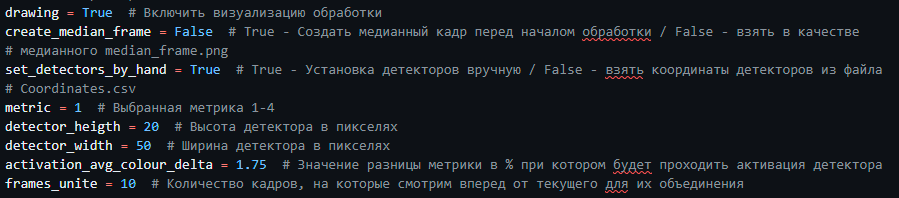
\includegraphics[width=0.9\textwidth]{images/detector_code.png}
\end{center}
\addcontentsline{toc}{section}{Настройка детектеров}


\newpage
\section*{Настройка "ViDeS"}
Для обработки видео, записанные в 30 кадров/сек, будем использовать "ViDeS"\\
Устанавливаем детекторы, примерно по 30 штук на каждую полосу, всего 89 штук
\begin{center}
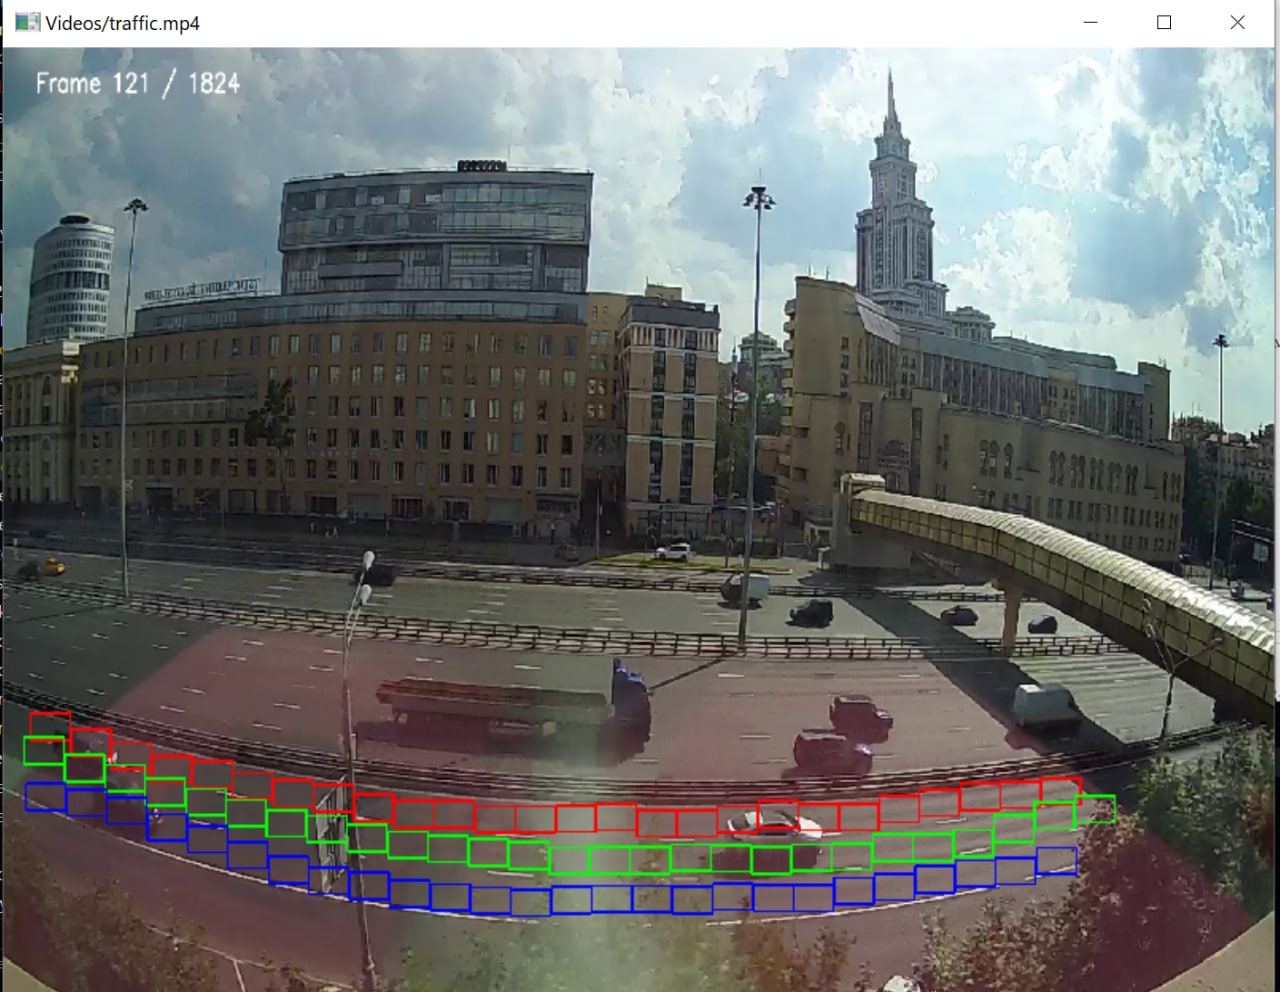
\includegraphics[width=0.8\textwidth]{images/vides_89_detectors.jpg}
\end{center}
После завершения программы, получаем .csv файлы с заполненными данными
Пример данных, содержащиеся в MetricValues.csv
\begin{center}
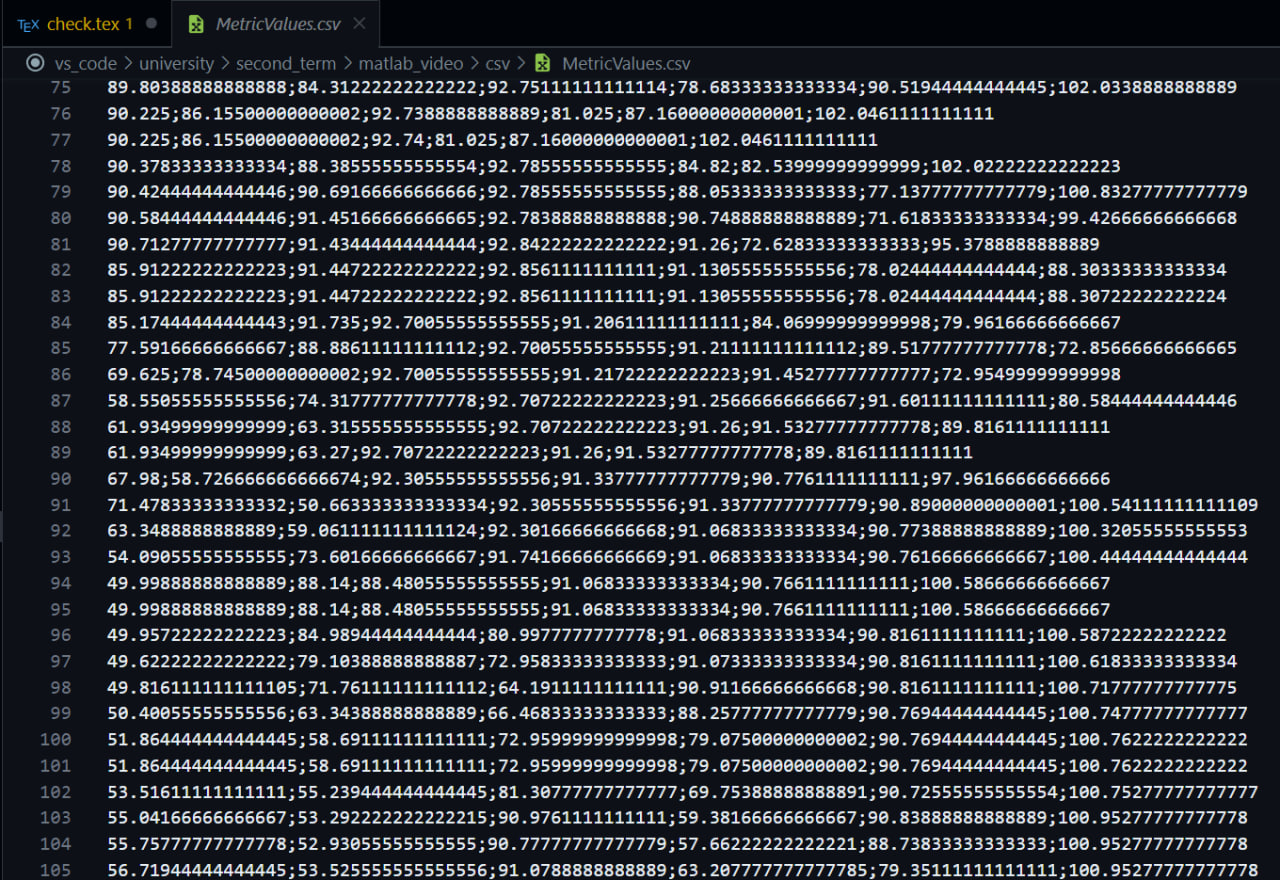
\includegraphics[width=0.9\textwidth]{images/vides_data.jpg}
\end{center}
\addcontentsline{toc}{section}{Настройка ViDeS}



\newpage
\section*{Первоначальный запуск "ViDeS"}
Перед запуском нужно поместить видеофайлы для обработки в папку Videos
и установить рекомендуемые параметры
\begin{enumerate}
    \item drawing: True
    \item createMedianFrame: True
    \item setDetectorsByHand: True
    \item metric: 1
\end{enumerate}
После завершения обработки программа заполняет файлы данными
\begin{enumerate}
    \item MetricValues.csv: значения выбранной метрики для каждого детектора для каждой полосы и каждой кадрах
    \item RawDetections.csv: неотфильтрованные значения активации каждого детектора, каждой полосы и кадра
    \item FilteredDetections.csv: отфильтрованные значения активации детектора для frameUnits
\end{enumerate}
\addcontentsline{toc}{section}{Первоначальный запуск ViDeS}


\section*{Построение гистограммы длин автомобилей}
Для построения всех графиков мы будем использовать полученные данные и пакет математических программ Matlab

Построили гистограмму для транспортных средств, которая показывает, сколько кадров машина находилась на детекторе\\
Благодоря этому мы может определить скорость машины и всего потока в целом
\begin{center}
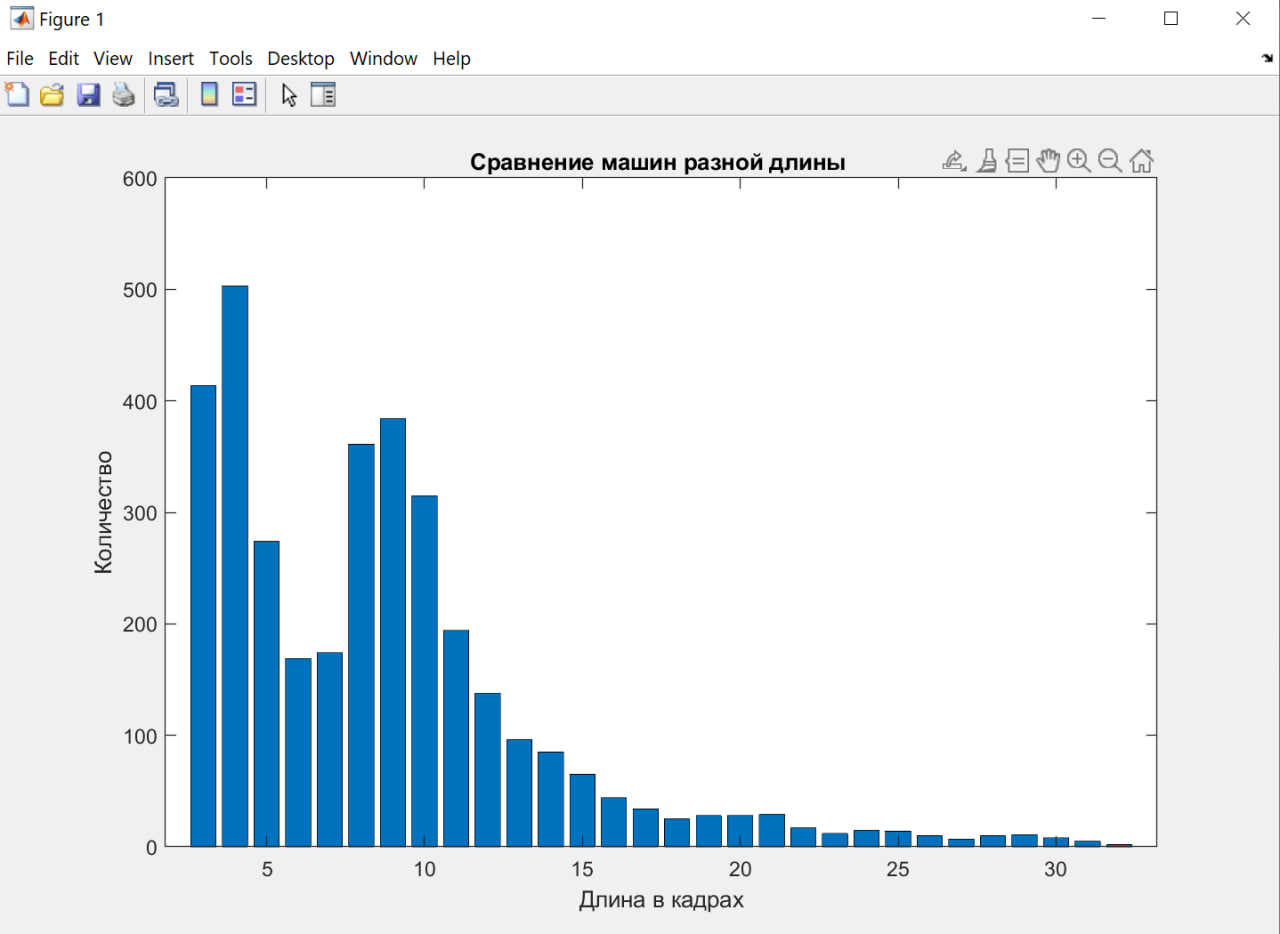
\includegraphics[width=0.9\textwidth]{images/histogram.jpg}
\end{center}
\begin{center}
Были взяты 3 датчика, по одному на каждой линии
\end{center}
\addcontentsline{toc}{section}{Построение гистограммы длин автомобилей}

\newpage
\section*{Построение графиков среднего цвета}
Для трех детекторов строим график среднего цвета, для первой и последней минуты.
По графику мы можем отследить динамику изменения цвета
\begin{center}
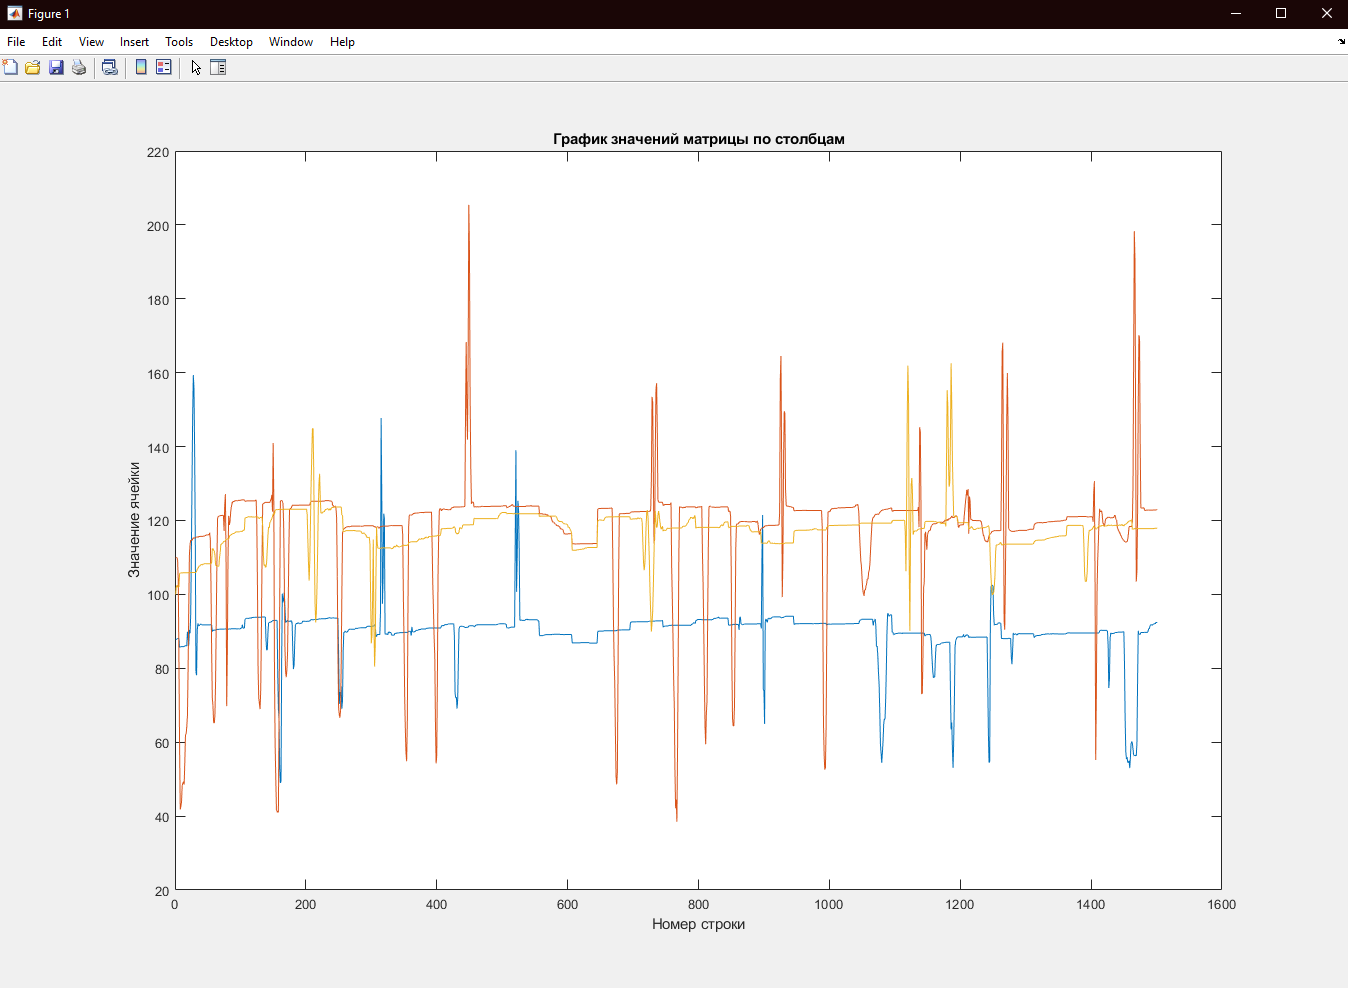
\includegraphics[width=0.9\textwidth]{images/median_color_first.png}
\end{center}
\begin{center}
График первой минуты
\end{center}
\begin{center}
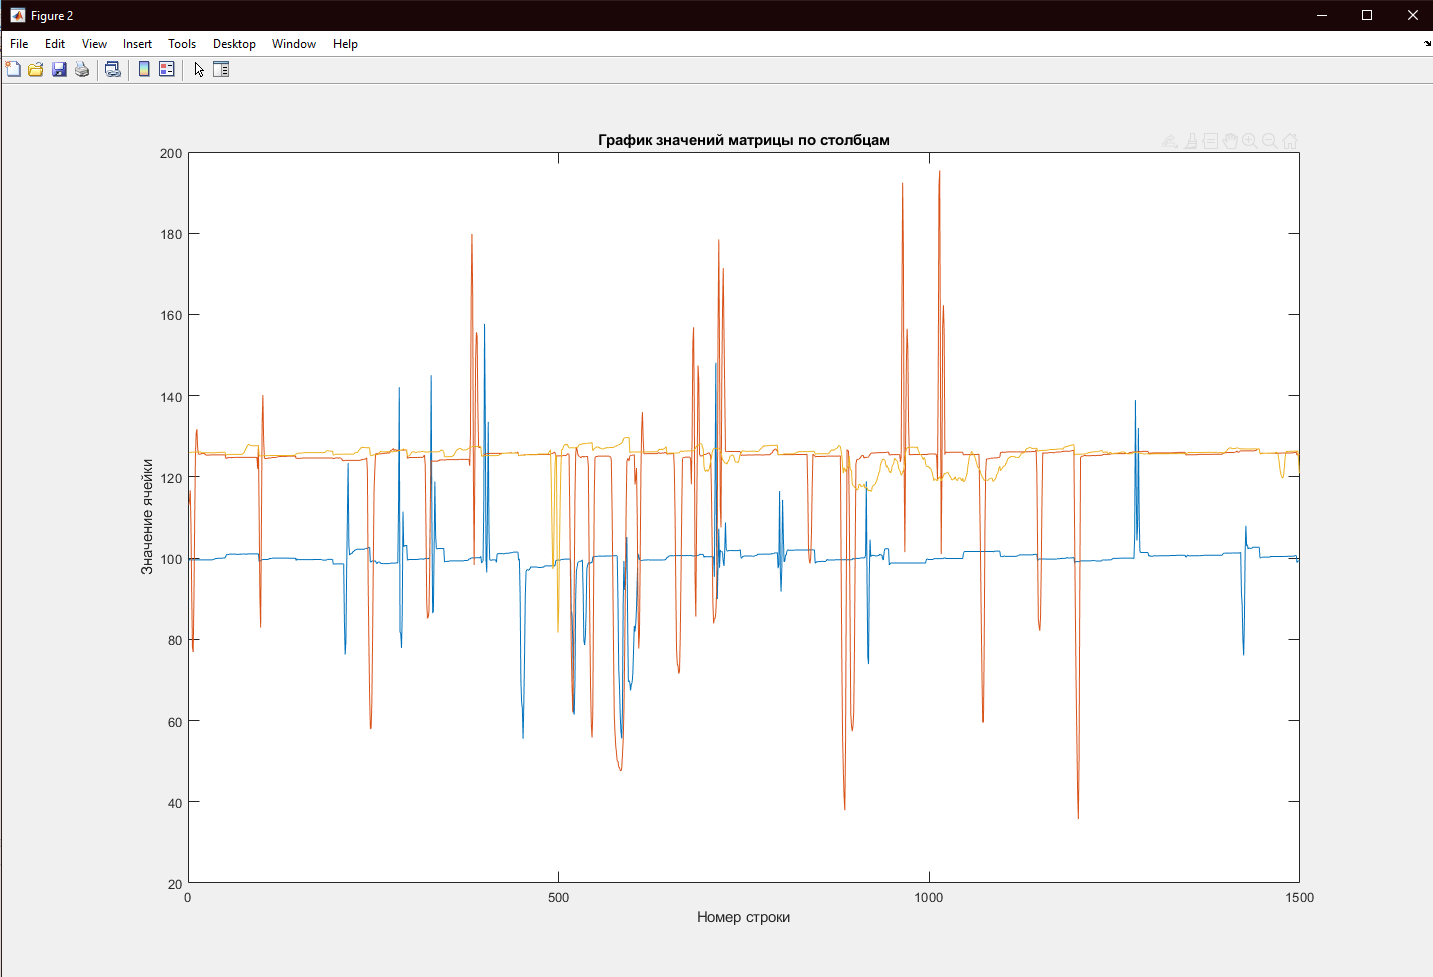
\includegraphics[width=0.9\textwidth]{images/median_color_last.png}
\end{center}
\begin{center}
График последней минуты
\end{center}
\addcontentsline{toc}{section}{Построение графиков среднего цвета}


\newpage
\section*{Построение бинаризированных графиков}
Для этих же датчиков строим бинаризированные графики, для первой и последней минуты\\
По ним мы сможем определить, в каких кадрах детекторы фиксировали машину
\begin{center}
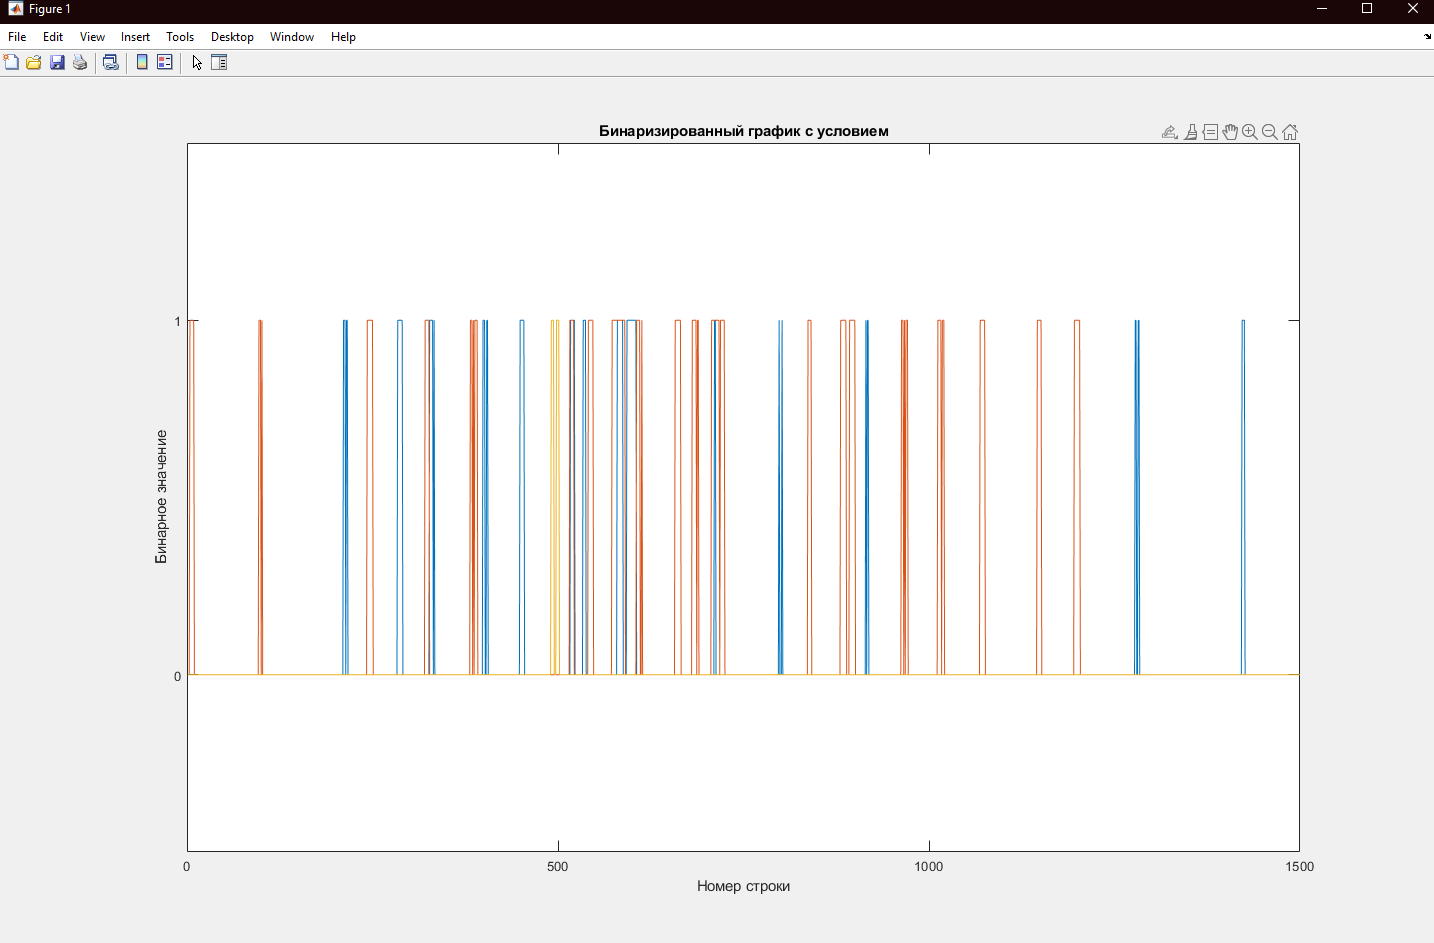
\includegraphics[width=0.9\textwidth]{images/binary_first.png}
\end{center}
\begin{center}
График первой минуты
\end{center}
\begin{center}
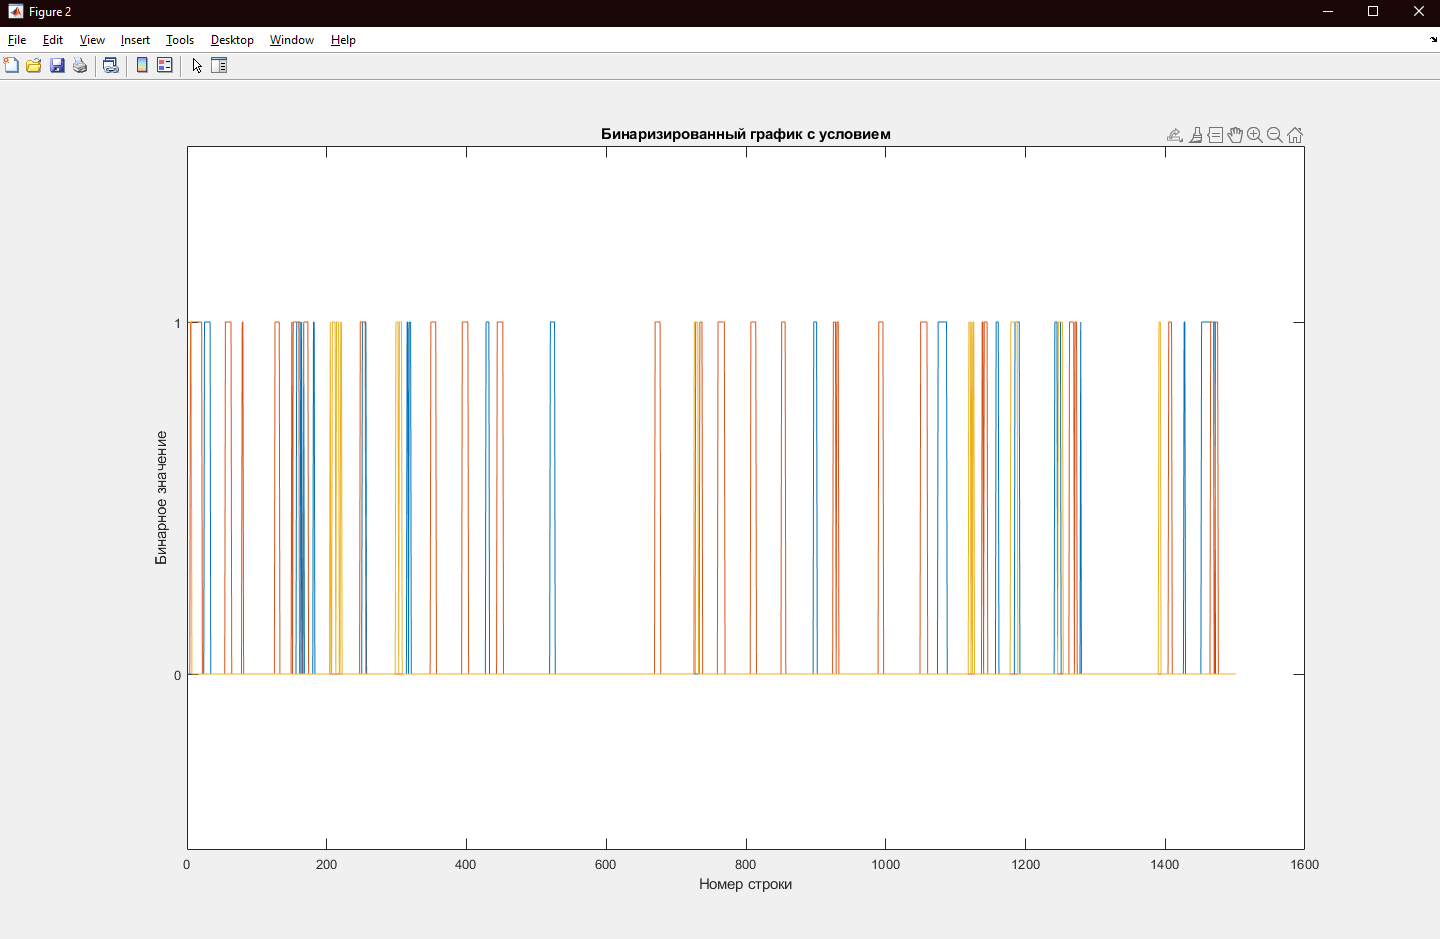
\includegraphics[width=0.9\textwidth]{images/binary_last.png}
\end{center}
\begin{center}
График последней минуты 
\end{center}
\addcontentsline{toc}{section}{Построение бинаризированных графиков}


\newpage
\section*{Построение совмещенных графиков}
Построение совмещенных графиков, которые содержат в себе графики среднего цвета,
а также графики бинаризированные. В бинаризированных графиках значения
параметра 'y' были расширены с [0; 1] до [0; 255], для улучшения наглядности
\begin{center}
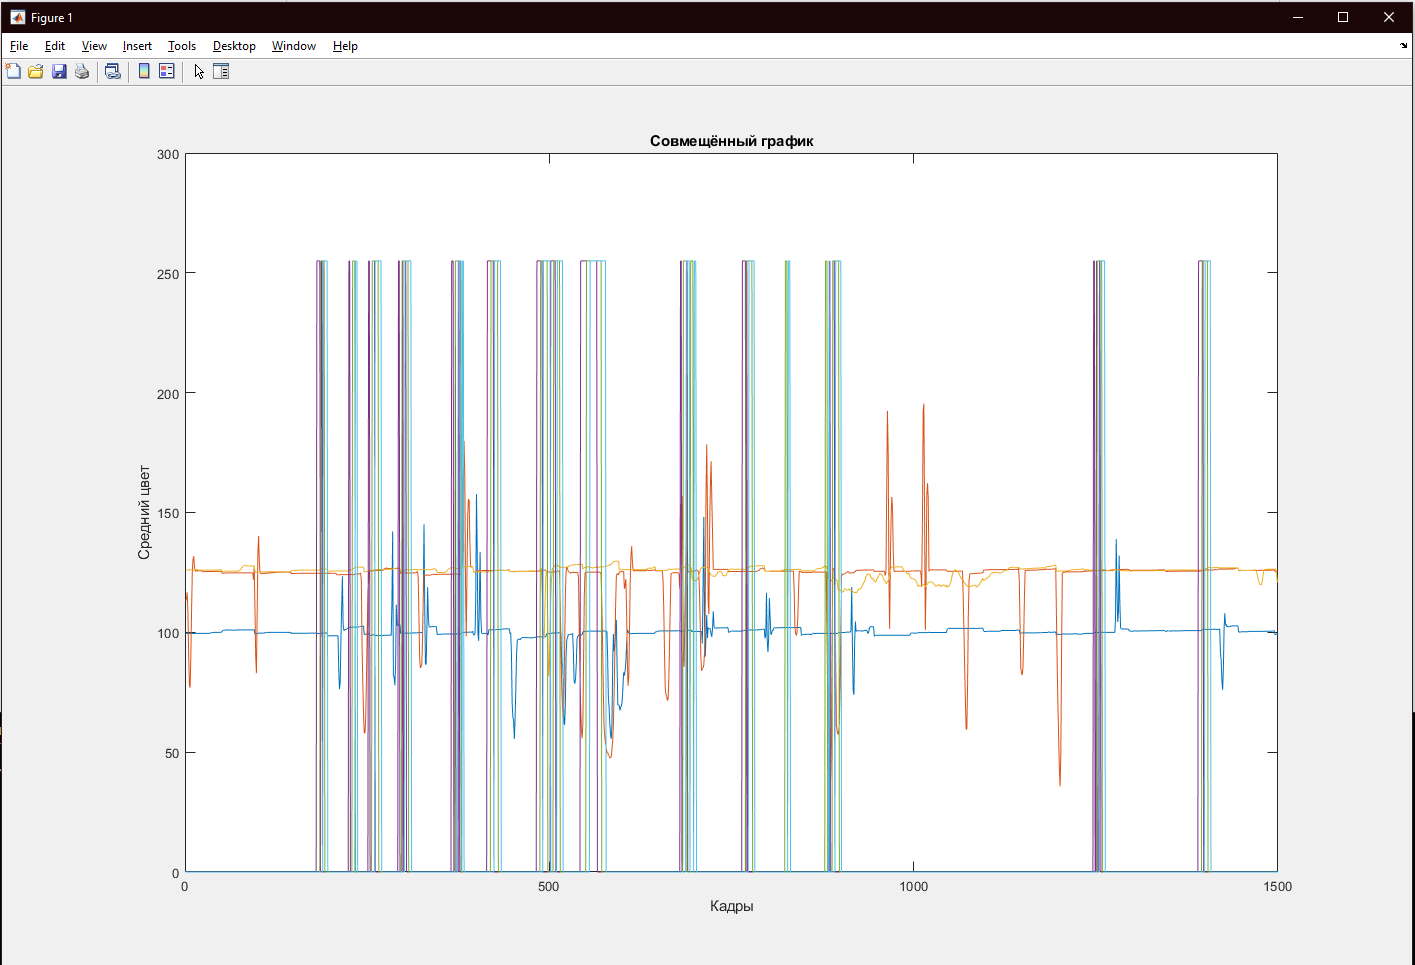
\includegraphics[width=0.9\textwidth]{images/merge_first.png}
\end{center}
\begin{center}
Совмещенные графики первой минуты
\end{center}
\begin{center}
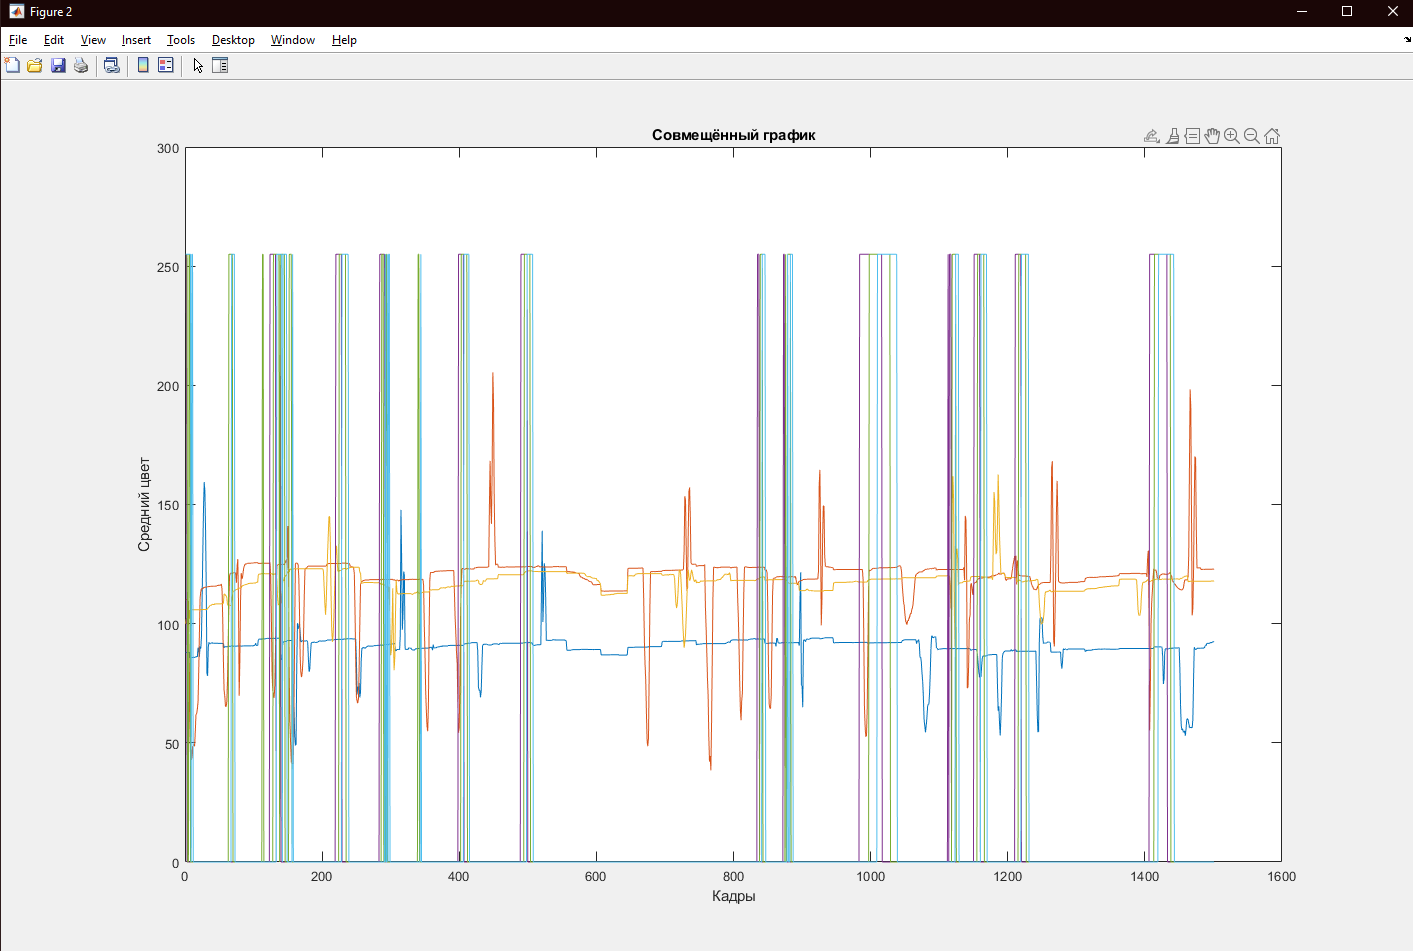
\includegraphics[width=0.9\textwidth]{images/merge_last.png}
\end{center}
\begin{center}
Совмещенные графики последней минуты 
\end{center}
\addcontentsline{toc}{section}{Построение совмещенных графиков}


\newpage
\section*{Вывод}
В результате проделанной работы удалось выяснить принципы работы детекторов, а также их точность.
При помощи ручной и автоматической оценки мы смогли оценить погрешность детекторов.\\
Построенные гистограммы длин автомобилей помогают оценить скороть транспортных средств,
а бинаризированные и совмещенные графики показывают плотность траффика.\\
Благодоря этим данным мы может проектировать будущие потоки, и избегать пробок
\addcontentsline{toc}{section}{Вывод}
\newpage
\end{document}
